\section{Data Gathering}
The data used in this project was gathered by recording three different persons reading the same article from the website "www.tv2.dk". The voices was recorded using the software Audacity\footnote{http://sourceforge.net/projects/audacity/} and the Lame mp3 codex\footnote{http://lame.sourceforge.net/}. The data is then imported into matlab using the function \texttt{[data, Fs] = audioread(pathToFile)}. The data is then normalised by removing the mean of the data, and whitening the data. The files are in stereo and both channels are used by appending one channel to the other so to have one long array of data.

\section{Feature Extraction}
The Mel Frequency Cepstral Coefficient method is commonly used to extract features in speech and speaker recognition. The methods provides features that are useful for classifying linguistic content. The basis is that the speech from humans is uniquely filtered by the shape of the vocal tract, tongue, teeth etc\footnote{http://practicalcryptography.com/miscellaneous/machine-learning/guide-mel-frequency-cepstral-coefficients-mfccs/ - retrieved 4 june 2015}. 

MFCCs are found using a series of steps as can be seen in figure \ref{fig:MFCCsteps}.
\begin{figure}[H]
\centering
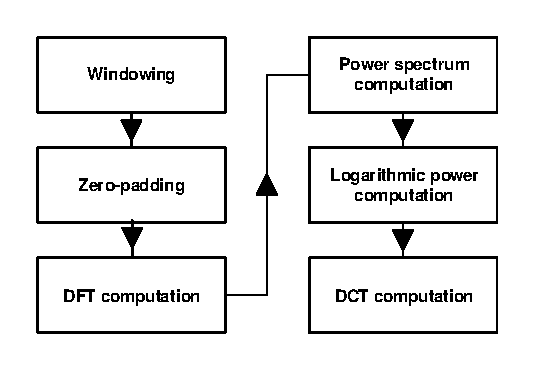
\includegraphics[scale=1]{billeder/MFCCsteps}
\caption{MFCC steps}
\label{fig:MFCCsteps}
\end{figure}
The figure has been derived from the article \cite{Sahidullah2012}. The steps can be described as follows:
\begin{enumerate}
\item Windowing
\item Zero-padding
\item DFT
\item Power spectrum
\item Logarithmic power
\item DCT
\end{enumerate}

Math\\

How we use it\\

\section{Features}

Size and number of features and stuff.

%------------------------------------------------